\documentclass{article}

\textwidth=6.5in
\textheight=8.5in
\voffset=-54pt
\oddsidemargin=0in
\evensidemargin=0in
\setlength{\parskip}{8pt}
\setlength{\parindent}{0pt}

\usepackage[normalem]{ulem}

\usepackage{amsmath, amssymb}
\usepackage{ifthen}

\usepackage[inline]{enumitem}
\setlist{topsep=0pt}

\usepackage{xcolor}
\usepackage[pdftex]{graphicx}

\usepackage{siunitx}
\sisetup{per-mode=fraction}

% change hyperref options
\PassOptionsToPackage{hyphens}{url}
\usepackage[bookmarks,colorlinks,linkcolor=black,citecolor=blue,pdfstartview=FitH,urlcolor=black]{hyperref}
\hypersetup{pdfpagemode=UseNone}

\usepackage{graphicx}
\usepackage{multicol}
\usepackage{framed}
\usepackage{array}
\usepackage{icomma}
\usepackage{diffcoeff}

\usepackage{soul}

\usepackage{pgfplots}
\pgfplotscreateplotcyclelist{mycolor}{%
  black, blue, red, green!70!black,magenta,
  purple, cyan, orange
}
\pgfplotsset{
  cycle list name=mycolor,
  axis lines=middle,
  every axis plot/.style={no marks, thick},
  every axis/.style={
    enlarge x limits=false,
    enlarge y limits=auto,
    xlabel style={at={(current axis.right of origin)},anchor=west},
    ylabel style={at={(current axis.above origin)},anchor=south},
    % extra x and y ticks for asymptotes
    extra x tick style={grid=major, grid style={dashed,black}},
    extra y tick style={grid=major, grid style={dashed,black}},
    /pgf/number format/1000 sep={},
  },
  tick label style = {font=\footnotesize, fill=white, inner sep=0pt},
  xticklabel shift=1pt,    
  scaled ticks=false,
  scaled y ticks=false,
  unbounded coords=jump,
  samples=101,
  minor tick length=0,
  scatter/classes={
    open={mark=*,draw=black,fill=white, mark size=2, thin},
    closed={mark=*,draw=black,fill=black, mark size=2, thin}
  },
  compat=1.18
}

\usepackage{tikz}
\usetikzlibrary{
  % enables the snake paths
  decorations.pathmorphing,%
  % enables bigger arrows
  decorations.markings,%
  decorations.pathreplacing,%
  decorations.text,%
  calc,%
  patterns,%
  shapes.geometric,%
  arrows,
  decorations.shapes,
  positioning,
  plotmarks,
}
\tikzset{>=latex} % sets default arrow type in tikz
\tikzset{font=\small}

\interfootnotelinepenalty=10000
\renewcommand{\thefootnote}{(\arabic{footnote})}

\usepackage{multirow, bigdelim}

\newcommand\iscurrentenumi[1]{%
  \ifthenelse{\equal{#1}{\theenumi}}{}{#1}}
\setenumerate[1]{ref=\#\arabic*}
\setenumerate[2]{ref=\protect\iscurrentenumi{\theenumi}(\alph*)}
\newcommand\enumiiprefix[2]{%
  \ifthenelse{{\equal{#1}{\theenumi}}\AND{\equal{#2}{(\alph{enumii})}}}{}{}%
  \ifthenelse{{\equal{#1}{\theenumi}}\AND{\NOT{\equal{#2}{(\alph{enumii})}}}}{#2}{}%
  \ifthenelse{\equal{#1}{\theenumi}}{}{#1#2}%
}
\setenumerate[3]{ref=\protect\enumiiprefix{\theenumi}{(\alph{enumii})}\roman*}

\definecolor{ideacolor}{rgb}{0.7,0,0}
\newcommand{\ideas}[1]{\color{ideacolor} #1 \color{black}}
\newcommand{\ideacolor}{maroon}

\newcommand{\outside}[1]{
    \fcolorbox{red}{white}{#1}
}

\newcommand{\inside}[1]{
    \fcolorbox{blue}{white}{#1}
}

\newlength{\tipmargin}
\makeatletter
\newcommand{\version}[2]{\ifthenelse{\equal{#1}{Mb}}{#2}{}}

\renewenvironment{framed}{
  \setlength{\tipmargin}{\textwidth-\linewidth}
  \advance\@totalleftmargin-\tipmargin
  \def\FrameCommand{\hspace{\tipmargin}\fbox}%
  \advance\linewidth\tipmargin
  \MakeFramed {\advance\hsize-\width \FrameRestore}%
}
{\endMakeFramed}

\makeatother

\newlength{\highlightwidth}
\newcommand{\highlight}[1]{\setlength{\highlightwidth}{\linewidth}%
  \addtolength{\highlightwidth}{-55pt}%
  \hspace{24pt}\begin{minipage}[t]{\highlightwidth} \setlength{\parskip}{8pt} #1 \end{minipage}\hspace{24pt}}

\definecolor{purple}{rgb}{0.5,0,1.0}

\newcommand{\textbook}[0]{\href{http://isites.harvard.edu/fs/docs/icb.topic1511355.files/fullbook.pdf}{textbook}}

% change to \usepackage[sols]{handout} to see solutions
% change to \usepackage[notes]{handout} to see notes
\usepackage[]{handout}
\renewcommand{\workshopnote}{CA Notes.}    

\begin{document}

\htitle{Worksheet 1 - The Chain Rule}
\begin{problemonly}
    \begin{framed}

You should be able to:

\begin{itemize}[topsep=0pt,partopsep=0pt,parsep=8pt,itemsep=0pt]

\item You should be able to use the Chain Rule to find the derivative of
  the composition of two functions.

\item You should understand why the Chain Rule makes sense in a real-world
  problem (such as {{\#1}} on {the worksheet ``The Chain Rule''}).

\item You should be comfortable looking at a function and determining its
  structure: is it a product?  A composition?  (If so, what is the outer
  function?)

\end{itemize} 

    \end{framed}
\end{problemonly}

\begin{enumerate}
\item {\bf Warm-up:} On your problem set last night, you reviewed compositions of functions. Decompose each of the functions below so that $h(x) = f(g(x))$.  

\begin{enumerate}
  \item \label{chain-rule-decompose-1-1} $h(x) = (10x^2+4)^2$ can be written as
    $f(g(x))$ with $g(x) = 10x^2+4$ and $f(u) = \fitb{0.75in}{u^2}$
    \pspace{12pt}

     \item \label{chain-rule-decompose-1-2} $h(x) = (2x+5)^{1/2}$ can be written as
    $f(g(x))$ with $g(x) = \fitb{0.75in}{2x+5}$ and $f(u) = \fitb{0.75in}{u^{1/2}}$
    \pspace{12pt}

  \item $h(x) =\displaystyle \frac{1}{3x}$ can be written as $f(g(x))$
    with $g(x) = 3x$ and $f(u) = \fitb{0.75in}{\frac{1}{u}}$
    \pspace{12pt}

    \item $j(x) =\displaystyle \frac{1}{(2x+5)^{1/2}}$ can be written as $f(g(h(x)))$\\
    
    with $h(x) = \fitb{0.75in}{2x+5}$, $g(u) = \fitb{0.75in}{\sqrt{u}}$ and $f(v) = \fitb{0.75in}{\frac{1}{v}}$
    \pspace{12pt}
    \end{enumerate}
    
\item 
  \note{I'll use this to try to convince them that the Chain Rule is
    reasonable.}

  Composition of functions allows us to make new models from old ones without starting from scratch. Here is an example: A rainwater collection tank is shaped so that 
  when the tank is filled with rainwater,
  the height of water in the tank can be measured. 
\begin{enumerate}
\item Which quantities are varying in this problem?
\begin{problemonly}
    \vfill
\end{problemonly}
\begin{solution}
    Volume of rainwater, height of rainwater in the water tank
\end{solution}

  \item Right away this description relates which two quantities and how? (Fill in the blank.)\\
  
  $\fitb{1in}{height}$ depends on $\fitb{1in}{height}$.

  \item Consider what happens in a rainstorm. As time passes, describe how we would expect the quantities to change?

  \begin{problemonly}
      \vfill
  \end{problemonly}
  (Fill in the blank.) This now introduces time. How are these three quantities related? \\
  
  $\fitb{1in}{height}$ depends on $\fitb{1in}{volume}$, which now depends  on $\fitb{1in}{time}$.

  \begin{solution} As time passes, the volume of water in the tank increases, and so the height of water in the tank is also increasing.
  \end{solution}


  \item Let's explore this connection and how it relates these quantities' rates of change: if you know that at a given moment in time, rainwater is pouring into the tank at 2 mL/s and you know that each additional mL causes the height of the water to increase by 0.2 mm, determine how height is changing as time passes.
  \begin{problemonly}
      \vfill
  \end{problemonly}

  \begin{solution}
      
  \end{solution}
 
  \item This connection between the instantaneous rates of change of functions in a composition is known as {\bf The Chain Rule}.  There are a few ways we use notation to describe this relationship.  \\

  Fill in the blank, then annotate with each symbol's meaning: 
  Given that height $h$, was a function of volume $v$, and $v$ was a function of time $t$, we can calculate the instantaneous rate of change of height $h$ with respect to time $t$:
  $$\displaystyle \frac{dh}{dt} = (\fitb{1in}{\frac{dh}{dv}})\cdot (\fitb{1in}{\frac{dv}{dt}})$$
  \begin{problemonly}
 \vspace{.5in}
 \end{problemonly}

Let $h = f(v)$, that is, height is a function of volume. Let $v=g(t)$, that is, volume is a function of time. Given these formal definitions, we could now describe the relationship between height and time as a composition, written $h=f(g(t))$. In which case, the same calculation to find how height is changing with respect to time could be written:

$$\frac{d}{dt} f(g(t)) = \fitb{1in}{f'(g(t))}\cdot \fitb{1in}{g'(t)} $$

\begin{problemonly}
 \vspace{.5in}
 \end{problemonly}

  \end{enumerate}



\begin{framed}
    \textbf{The Chain Rule:} Given a composition of functions $f(g(t))$, the derivative is:
    $$\dfrac{d}{dt}[f(g(t))]= \solonly{f'(g(t))\cdot g'(t) }
    \hspace{1.5 in} \text{or} \hspace{.5 in} \dfrac{df}{dt} = 
    \solonly{\dfrac{df}{dg} \cdot \dfrac{dg}{dt}}
    $$ 
\end{framed}

\pspace{\newpage}

\item 
  
  This allows us the ability to differentiate more efficiently than before and tackle new functions.
  \begin{enumerate}

  \item

     \begin{problem}[\stretch{0.5}]
      From earlier in the week: $a(s) = (3s + 1)^2$. Find $a'(s)$ without first expanding.
    \end{problem}

    \begin{solution}
      We can decompose $h(x)$ as $f(g(x))$ with $g(x) = 7x^2 + 3$ and
      $f(x) = \ln x$.  Then, $g'(x) = 14 x$ and $f'(x) = \frac{1}{x}$, so
      $h'(x) = f'(g(x)) g'(x) = f'(7x^2 + 3) g'(x) = \boxed{\frac{1}{7x^2
          + 3} \cdot 14x}$ by the Chain Rule. 
    \end{solution}

\item $k(r)=\dfrac{1}{2r^7+1}$. Find $k'(r)$.
\begin{problemonly}
    \vfill
\end{problemonly}

  \item
    \begin{problem}[\vfill]
     $h(x) = \pi^3 (7x + 3)^{10}$
    \end{problem}

    \begin{solution}
      Since $\pi^3$ is a constant,
      \begin{align*}
        h'(x) = {} & \pi ^3\cdot \frac{d}{dx} \left(\fcolorbox{red}{white}{$\displaystyle \fcolorbox{blue}{white}{$\displaystyle  \left(7 x+ 3\right)$}^ { 10} $}\right) \\
        = {} & \pi ^3\cdot 10 \left(7 x+ 3\right)^ { 9} \cdot 7
      \end{align*}
    \end{solution}

  \item
    \begin{problem}[\stretch{0.5}]
      $y = \dfrac{\sqrt{x^2 + 1}}{\pi}$. Find $\dfrac{dy}{dx}$
    \end{problem}

    \begin{solution}
      We can rewrite $y$ as $\frac{1}{\pi} \sqrt{x^2 + 1}$; since
      $\frac{1}{\pi}$ is a constant,
      \begin{align*}
        y' = {} \frac{1}{\pi} \frac{d}{dx}
        \left(\fcolorbox{red}{white}{$\displaystyle
            \fcolorbox{blue}{white}{$\displaystyle  \left(x^2 + 1
              \right)$}^ { \frac{1}{2}} $}\right) = {} & \frac{1}{\pi} \cdot
        \frac{1}{2}
        \left(x^2 + 1 \right)^ { -\frac{1}{2}} \cdot
        \frac{d}{dx}\left(x^2 + 1 \right) \\ 
        = {} & \frac{1}{2\pi} \left(x^2 + 1 \right)^ { -\frac{1}{2}}
        \left(2x \right) 
      \end{align*}
    \end{solution}

  \item

    \begin{problem}[]
      The Chain Rule can also be used in combination with other rules.
      \end{problem}
      \begin{enumerate}
          \item
   \begin{problem}[\vfill]
      From earlier in the week, $\displaystyle u(r) = \frac{5r + 3}{2r^7 + 1}$. Find $\dfrac{du}{dr}$ without using the Quotient Rule.
    \end{problem}

    \begin{solution}
      We can decompose $e^{t^3}$ as $f(g(t))$ with $g(t) = t^3$ and $f(t)
      = e^t$.  Then, the Chain Rule says that $\frac{d}{dt} \left(e^{t^3}
      \right) = f'(g(t)) g'(t) = e^{t^3} \cdot 3t^2$, so $q'(t) =
      \boxed{3t^2 e^{t^3} - 12 e^2}$.

      Instead of writing out functions $f(t)$ and $g(t)$, we'll often
      write that we're going to use the Chain Rule simply by putting a red
      box around where we're going to use the Chain Rule ($e^{t^3}$ in
      this case) and then putting a blue box around the inner function
      $g(t)$: 
      \begin{align*}
        q'(t) &= \frac{d}{dt} \left(\fcolorbox{red}{white}{$\displaystyle
            e^ { \fcolorbox{blue}{white}{$\displaystyle t^ { 3} $}}
            $} - 12 e^2 t \right) \\ 
        &= e^ { t^ { 3} } \cdot 3 t^ { 2} -12 e^2
      \end{align*}
    \end{solution}
    
      \item 
      \begin{problem}[\vfill] Find $f'(x)$ if $\displaystyle f(x) =  \frac{x^2}{(x-2)(3x+5)}
      $. 
    \end{problem}

    \begin{solution}
      We can first use log rules to rewrite $f(x)$:
      \begin{align*}
        f(x) &= \ln x^2 - \ln [(x - 2) (3x + 5)] \\
        &= 2 \ln x - \left[ \ln(x - 2) + \ln (3x + 5)
        \right] \\
        &= 2 \ln x - \ln(x - 2) - \ln (3x + 5)
      \end{align*}
      Now let's differentiate, using the Chain Rule:
      \begin{align*}
        f'(x) = {} & 2 \cdot \frac{d}{dx} \left(\fcolorbox{red}{white}{$\displaystyle \ln\left(\fcolorbox{blue}{white}{$\displaystyle x$}\right)$}\right)-\frac{d}{dx} \left(\fcolorbox{red}{white}{$\displaystyle \ln\left(\fcolorbox{blue}{white}{$\displaystyle x-2$}\right)$}\right)-\frac{d}{dx} \left(\fcolorbox{red}{white}{$\displaystyle \ln\left(\fcolorbox{blue}{white}{$\displaystyle 3x+ 5$}\right)$}\right) \\
        = {} & 2\cdot \frac{1}{x}\cdot 1-\frac{1}{x-2}\cdot 1-\frac{1}{3x+ 5}\cdot 3
      \end{align*}
    \end{solution}
\end{enumerate}

  \end{enumerate}
\begin{problemonly}
    \newpage
\end{problemonly}
\item 

  \begin{enumerate}
  \item 
    \begin{problem}[\stretch{2}]
      How does the graph of $(x+5)^2$ relate to the graph of $x^2$?
      Use the Chain Rule to differentiate $(x+5)^2$.  Is your answer
      consistent with the graph and what you know about the derivative of
      $x^2$?
    \end{problem}

    \begin{solution}
      The graph of $\ln(x + 5)$ is simply the graph of $\ln x$ shifted 5
      units to the left.  Graphically, this means that the derivative of
      $\ln(x + 
      5)$ should be the derivative of $\ln x$ shifted left by 5.  That is,
      it should be $\frac{1}{x}$ shifted left by $5$, which has the
      formula $\frac{1}{x + 5}$. 

      Let's check.  By the Chain Rule,
      \[ \frac{d}{dx} \left(\fcolorbox{red}{white}{$\displaystyle
          \ln\left(\fcolorbox{blue}{white}{$\displaystyle x+
              5$}\right)$}\right) = \frac{1}{x+ 5}\cdot 1 = \frac{1}{x +
        5},\]
      as we expected.        
    \end{solution}

  \item
    \begin{problem}[\vfill]
      More generally, if $c$ is a constant, how does the graph of $f(x +
      c)$ relate to the graph of $f(x)$?  What does the Chain Rule tell
      you about the derivative of $f(x + c)$?
    \end{problem}

    \begin{solution}
      More generally, 
      the graph of $f(x + c)$ is simply the graph of $f(x)$ shifted $c$
      units to the left, so we expect the derivative of $f(x + c)$ (which
      we write as $\frac{d}{dx} f(x + c)$) to be $f'(x)$ shifted $c$ units
      to the left, or $f'(x + c)$. 

      By the Chain Rule,     
      \[ \frac{d}{dx} \left(\fcolorbox{red}{white}{$\displaystyle
          f\left(\fcolorbox{blue}{white}{$\displaystyle x+
              c$}\right)$}\right) = f'\left(x+ c\right)\cdot 1 = f'(x +
      c),\] as we expected. 
    \end{solution}    

  \end{enumerate}

  \item 
  \begin{problem}[\vfill]
    You are given the following information about three functions
    $f$, $g$, and $h$.
    \begin{align*}
      h(1) &= 2 & g(2) &= 3 & f'(3) &= 6 \\
      h'(1) &= 4 & g'(2) &= 5 
    \end{align*}
    If $r(x) = f(g(h(x)))$, do you have enough information to find
    $r'(1)$?  If so, compute it. If not, what additional information do
    you need?
  \end{problem}

  \begin{solution}
    First, let's find $r'(x)$:
    \begin{align*}
      r'(x) = {} & \frac{d}{dx}
      \left(\fcolorbox{red}{white}{$\displaystyle
          f\left(\fcolorbox{blue}{white}{$\displaystyle
              g\left(h(x)\right)$}\right)$}\right) \\
      = {} & f'\left(g\left(h(x)\right)\right)\cdot
      \frac{d}{dx} \left(\fcolorbox{red}{white}{$\displaystyle
          g\left(\fcolorbox{blue}{white}{$\displaystyle
              h(x)$}\right)$}\right) \\ 
      = {} & f'(g(h(x)))\cdot
      g'(h(x))\cdot h'(x)
    \end{align*}
    Plugging in $x = 1$, 
    \begin{align*}
      r'(1) &= f'(g(h(1))) g'(h(1)) h'(1) \\
      &= f'(g(2)) g'(2) \cdot 4 \\
      &= f'(3) \cdot 5 \cdot 4 \\
      &= 6 \cdot 5 \cdot 4 \\
      &= \boxed{120}
    \end{align*}
    (So, we did have enough information to find $r'(1)$.)
  \end{solution}


\item 

  \note{Here, they'll need to remember that the derivative at a point can
    be visualized as slope of a tangent line.  This fact is always worth
    reinforcing!}
    
  \begin{problem}
    Here are graphs of two functions, $f(x)$ and $g(x)$.  If $h(x) =
    f(g(x))$, what is $h'(1)$?

    \begin{tabular}{ccc}
      $f(x)$ & & $g(x)$ \\ \\ 
      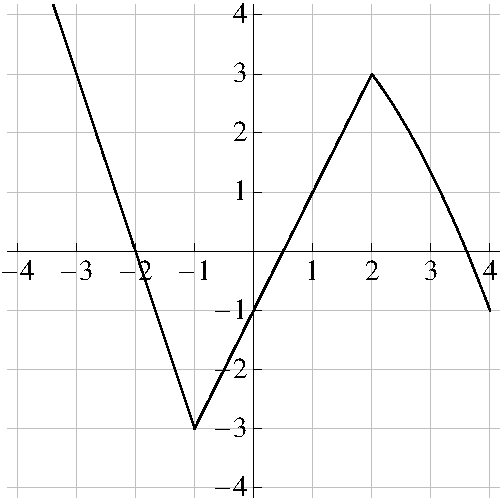
\includegraphics[width=1.75in]{images/chain-rule-graphical-f.pdf} & 
      \hspace{0.25in} & 
      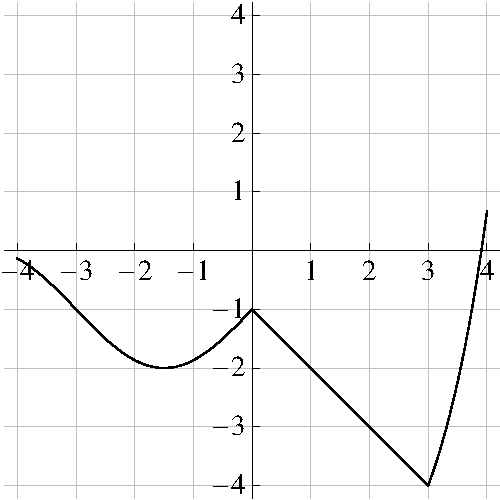
\includegraphics[width=1.75in]{images/chain-rule-graphical-g.pdf} 
    \end{tabular}
  \end{problem}

  \begin{solution}
    By the Chain Rule, $h'(1) = f'(g(1)) g'(1)$.  From the graph of $g$,
    we see that $g(1) = -2$ and $g'(1) = -1$.  Therefore, $h'(1) =
    -f'(-2)$.  From the graph of $f$, we see that $f'(-2) = -3$, so
    $h'(1)$ is equal to \fbox{3}.
  \end{solution}

\end{enumerate}


\end{document}